\newpage
\hypertarget{subSec:setupParser}{}
\subsection{Setting up the parser}
\genHeader

Our convention is that the \emph{code adapter} project we established in the previous step contains all tree-to-model transformation logic for the project.
Although the transformation \emph{could} be integrated directly in the corresponding metamodel (\texttt{Dic\-tion\-ary\-Language}), a separation makes sense here as
there could be \emph{different} code adapters for the \emph{same} language. 

To continue setting up the framework for our transformation, let's establish an ANTLR parser/unparser which will enable us to transform from tree-to-text (and
vice versa).

\begin{itemize}

\item[$\blacktriangleright$] Right-click on the generated \texttt{DictionaryCodeAdapter} folder and navigate to ``eMoflon/ Add Parser/Unparser''
(Fig~\ref{eclipse:contextParser}).\footnote{For presentation purposes, this context menu screenshot has been edited}

\vspace{0.5cm}

\begin{figure}[htpb]
\begin{center}
  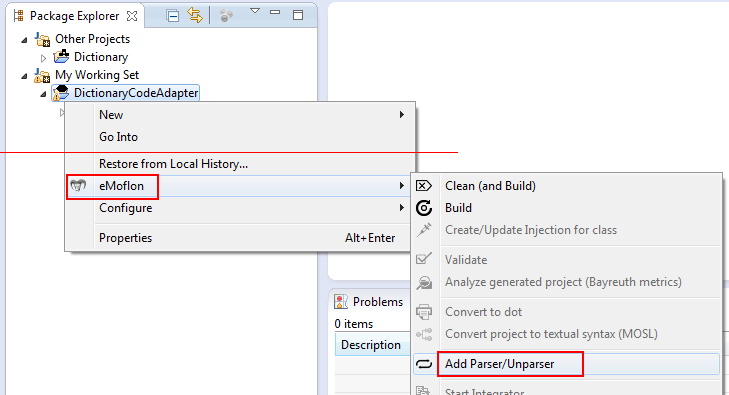
\includegraphics[width=0.8\textwidth]{eclipse_contextAddParserUnparser}
  \caption{Adding a new parser/unparser to a project}
  \label{eclipse:contextParser}
\end{center}
\end{figure}


\item[$\blacktriangleright$] In the parser settings window, enter \texttt{dictionary} as the \texttt{File exten\-si\-on}, and confirm that the \texttt{Create
Parser}, \texttt{Create Unparser}, and \texttt{ANTLR} options are selected as the corresponding technology for each case (Fig~\ref{eclipse:wizardParser}).
Affirm by pressing \texttt{Finish}.

\begin{figure}[htpb]
\begin{center}
  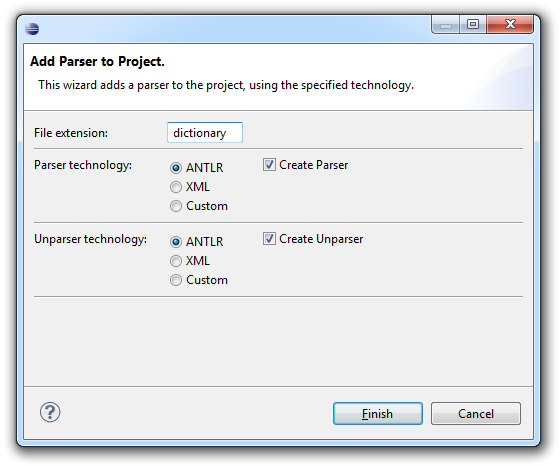
\includegraphics[width=0.8\textwidth]{eclipse_wizardParser}
  \caption{Parser/unparser settings}
  \label{eclipse:wizardParser}
\end{center}
\end{figure}


\item[$\blacktriangleright$] If everything executed without error, parser and unparser stubs should be generated in the \texttt{src} package
(Fig.~\ref{eclipse:generatedParser}). In addition, a new \texttt{in} folder should appear under \texttt{instances}. 

\begin{figure}[htpb]
\begin{center}
  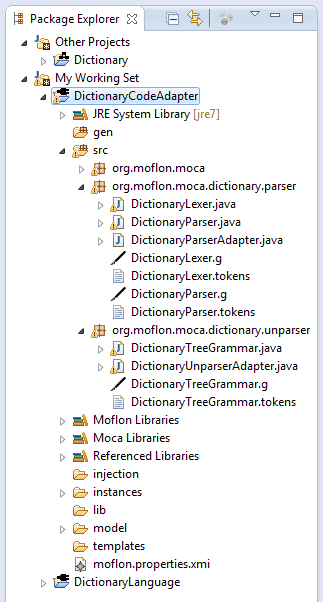
\includegraphics[width=0.4\textwidth]{eclipse_generatedParser}
  \caption{Generated stubs and derived files}
  \label{eclipse:generatedParser}
\end{center}
\end{figure}

\end{itemize}
